\documentclass{standalone}
\usepackage{tikz}
\usetikzlibrary{patterns, positioning}


\begin{document}
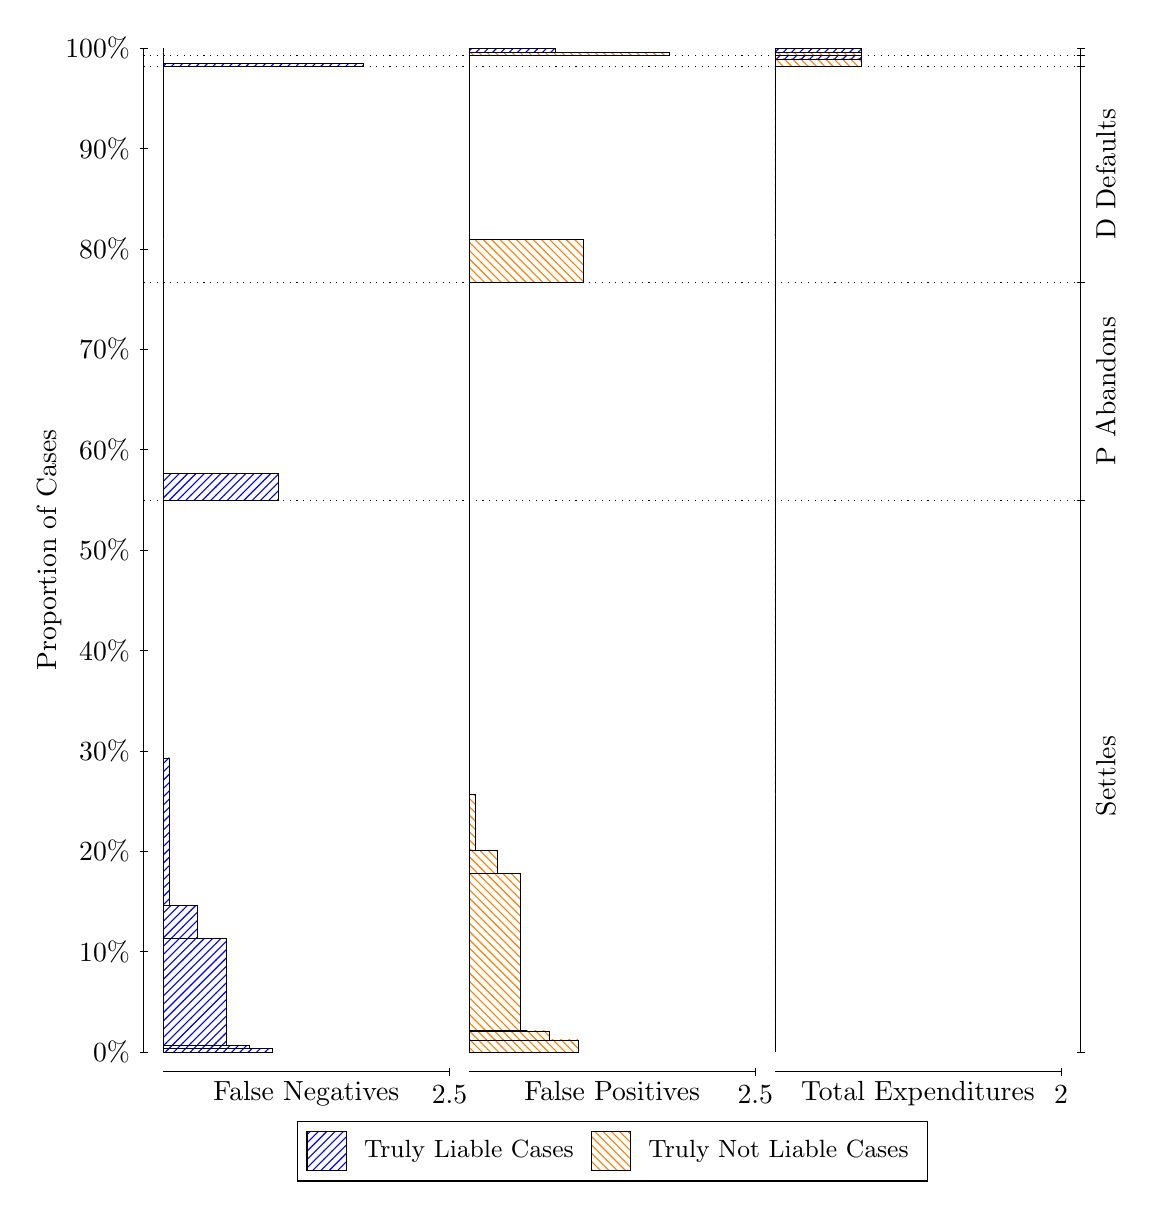
\begin{tikzpicture}
\draw[black, very thin] (1.5,1.75) -- (1.5,14.5);
\node[rotate=90, text=black, anchor=center] at (0.3, 8.125) {Proportion of Cases};
\draw[black, very thin] (1.45,1.75) -- (1.55,1.75);
\node[text=black, anchor=east] at (1.45, 1.75) {0\%};
\draw[black, very thin] (1.45,3.025) -- (1.55,3.025);
\node[text=black, anchor=east] at (1.45, 3.025) {10\%};
\draw[black, very thin] (1.45,4.3) -- (1.55,4.3);
\node[text=black, anchor=east] at (1.45, 4.3) {20\%};
\draw[black, very thin] (1.45,5.575) -- (1.55,5.575);
\node[text=black, anchor=east] at (1.45, 5.575) {30\%};
\draw[black, very thin] (1.45,6.85) -- (1.55,6.85);
\node[text=black, anchor=east] at (1.45, 6.85) {40\%};
\draw[black, very thin] (1.45,8.125) -- (1.55,8.125);
\node[text=black, anchor=east] at (1.45, 8.125) {50\%};
\draw[black, very thin] (1.45,9.4) -- (1.55,9.4);
\node[text=black, anchor=east] at (1.45, 9.4) {60\%};
\draw[black, very thin] (1.45,10.675) -- (1.55,10.675);
\node[text=black, anchor=east] at (1.45, 10.675) {70\%};
\draw[black, very thin] (1.45,11.95) -- (1.55,11.95);
\node[text=black, anchor=east] at (1.45, 11.95) {80\%};
\draw[black, very thin] (1.45,13.225) -- (1.55,13.225);
\node[text=black, anchor=east] at (1.45, 13.225) {90\%};
\draw[black, very thin] (1.45,14.5) -- (1.55,14.5);
\node[text=black, anchor=east] at (1.45, 14.5) {100\%};

\draw[black, very thin] (13.4,1.75) -- (13.4,14.5);
\draw[black, very thin] (13.35,1.75) -- (13.45,1.75);
\node[anchor=west] at (13.35, 1.75) {};
\draw[black, very thin] (13.35,8.7577) -- (13.45,8.7577);
\node[anchor=west] at (13.35, 8.7577) {};
\draw[black, very thin] (13.35,11.526) -- (13.45,11.526);
\node[anchor=west] at (13.35, 11.526) {};
\draw[black, very thin] (13.35,14.265) -- (13.45,14.265);
\node[anchor=west] at (13.35, 14.265) {};
\draw[black, very thin] (13.35,14.402) -- (13.45,14.402);
\node[anchor=west] at (13.35, 14.402) {};
\draw[black, very thin] (13.35,14.5) -- (13.45,14.5);
\node[anchor=west] at (13.35, 14.5) {};

\draw[black, very thin, pattern color=blue, pattern=north east lines] (1.75,1.75) rectangle (3.1307,1.7938);
\draw[black, very thin, pattern color=blue, pattern=north east lines] (1.75,1.7938) rectangle (2.84,1.8366);
\draw[black, very thin, pattern color=blue, pattern=north east lines] (1.75,1.8366) rectangle (2.5493,3.1903);
\draw[black, very thin, pattern color=blue, pattern=north east lines] (1.75,3.1903) rectangle (2.4767,3.1927);
\draw[black, very thin, pattern color=blue, pattern=north east lines] (1.75,3.1927) rectangle (2.186,3.6122);
\draw[black, very thin, pattern color=blue, pattern=north east lines] (1.75,3.6122) rectangle (1.8227,5.4859);
\draw[black, very thin, pattern color=orange, pattern=north west lines] (1.75,5.4859) rectangle (1.75,8.7577);
\draw[black, very thin, pattern color=blue, pattern=north east lines] (1.75,8.7577) rectangle (3.2033,9.1001);
\draw[black, very thin, pattern color=orange, pattern=north west lines] (1.75,9.1001) rectangle (1.75,11.526);
\draw[black, very thin, pattern color=orange, pattern=north west lines] (1.75,11.526) rectangle (1.75,12.067);
\draw[black, very thin, pattern color=blue, pattern=north east lines] (1.75,12.067) rectangle (1.75,14.265);
\draw[black, very thin, pattern color=blue, pattern=north east lines] (1.75,14.265) rectangle (4.2933,14.306);
\draw[black, very thin, pattern color=orange, pattern=north west lines] (1.75,14.306) rectangle (1.75,14.402);
\draw[black, very thin, pattern color=orange, pattern=north west lines] (1.75,14.402) rectangle (1.75,14.443);
\draw[black, very thin, pattern color=blue, pattern=north east lines] (1.75,14.443) rectangle (1.75,14.5);
\draw[black, very thin, pattern color=orange, pattern=north west lines] (5.6333,1.75) rectangle (7.014,1.9035);
\draw[black, very thin, pattern color=orange, pattern=north west lines] (5.6333,1.9035) rectangle (6.6507,2.0171);
\draw[black, very thin, pattern color=orange, pattern=north west lines] (5.6333,2.0171) rectangle (6.36,2.0207);
\draw[black, very thin, pattern color=orange, pattern=north west lines] (5.6333,2.0207) rectangle (6.2873,4.0145);
\draw[black, very thin, pattern color=orange, pattern=north west lines] (5.6333,4.0145) rectangle (5.9967,4.3074);
\draw[black, very thin, pattern color=orange, pattern=north west lines] (5.6333,4.3074) rectangle (5.706,5.0218);
\draw[black, very thin, pattern color=blue, pattern=north east lines] (5.6333,5.0218) rectangle (5.6333,8.7577);
\draw[black, very thin, pattern color=orange, pattern=north west lines] (5.6333,8.7577) rectangle (5.6333,11.184);
\draw[black, very thin, pattern color=blue, pattern=north east lines] (5.6333,11.184) rectangle (5.6333,11.526);
\draw[black, very thin, pattern color=orange, pattern=north west lines] (5.6333,11.526) rectangle (7.0867,12.067);
\draw[black, very thin, pattern color=blue, pattern=north east lines] (5.6333,12.067) rectangle (5.6333,14.265);
\draw[black, very thin, pattern color=orange, pattern=north west lines] (5.6333,14.265) rectangle (5.6333,14.361);
\draw[black, very thin, pattern color=blue, pattern=north east lines] (5.6333,14.361) rectangle (5.6333,14.402);
\draw[black, very thin, pattern color=orange, pattern=north west lines] (5.6333,14.402) rectangle (8.1767,14.443);
\draw[black, very thin, pattern color=blue, pattern=north east lines] (5.6333,14.443) rectangle (6.7233,14.5);
\draw[black, very thin, pattern color=orange, pattern=north west lines] (9.5167,1.75) rectangle (9.5167,5.0218);
\draw[black, very thin, pattern color=blue, pattern=north east lines] (9.5167,5.0218) rectangle (9.5167,8.7577);
\draw[black, very thin, pattern color=orange, pattern=north west lines] (9.5167,8.7577) rectangle (9.5167,11.184);
\draw[black, very thin, pattern color=blue, pattern=north east lines] (9.5167,11.184) rectangle (9.5167,11.526);
\draw[black, very thin, pattern color=orange, pattern=north west lines] (9.5167,11.526) rectangle (9.5167,12.067);
\draw[black, very thin, pattern color=blue, pattern=north east lines] (9.5167,12.067) rectangle (9.5167,14.265);
\draw[black, very thin, pattern color=orange, pattern=north west lines] (9.5167,14.265) rectangle (10.607,14.361);
\draw[black, very thin, pattern color=blue, pattern=north east lines] (9.5167,14.361) rectangle (10.607,14.402);
\draw[black, very thin, pattern color=orange, pattern=north west lines] (9.5167,14.402) rectangle (10.607,14.443);
\draw[black, very thin, pattern color=blue, pattern=north east lines] (9.5167,14.443) rectangle (10.607,14.5);
\draw[black, dotted] (1.5,8.7577) -- (13.4,8.7577);
\draw[black, dotted] (1.5,11.526) -- (13.4,11.526);
\draw[black, dotted] (1.5,14.265) -- (13.4,14.265);
\draw[black, dotted] (1.5,14.402) -- (13.4,14.402);
\draw[black, very thin] (1.75,1.5) -- (5.3833,1.5);
\node[text=black, anchor=north] at (3.5667, 1.5) {False Negatives};
\draw[black, very thin] (5.3833,1.45) -- (5.3833,1.55);
\node[text=black, anchor=north] at (5.3833, 1.45) {2.5};

\draw[black, very thin] (5.6333,1.5) -- (9.2667,1.5);
\node[text=black, anchor=north] at (7.45, 1.5) {False Positives};
\draw[black, very thin] (9.2667,1.45) -- (9.2667,1.55);
\node[text=black, anchor=north] at (9.2667, 1.45) {2.5};

\draw[black, very thin] (9.5167,1.5) -- (13.15,1.5);
\node[text=black, anchor=north] at (11.333, 1.5) {Total Expenditures};
\draw[black, very thin] (13.15,1.45) -- (13.15,1.55);
\node[text=black, anchor=north] at (13.15, 1.45) {2};

\node[text=black, centered, rotate=90] at (13.72, 5.2538) {Settles};
\node[text=black, centered, rotate=90] at (13.72, 10.142) {P Abandons};
\node[text=black, centered, rotate=90] at (13.72, 12.896) {D Defaults};



\draw (7.449999999999999,1.5) node[draw=none] (baseCoordinate) {};
\begin{scope}[align=center]
        \matrix[scale=0.5, draw=black, below=0.5cm of baseCoordinate, nodes={draw}, column sep=0.1cm]{
            \node[rectangle, draw, minimum width=0.5cm, minimum height=0.5cm, pattern color=blue, pattern=north east lines] {}; &
            \node[draw=none, font=\small, text=black] (B) {Truly Liable Cases}; &
            \node[rectangle, draw, minimum width=0.5cm, minimum height=0.5cm, pattern color=orange, pattern=north west lines] {}; &
            \node[draw=none, font=\small, text=black] (B) {Truly Not Liable Cases}; \\
            };
\end{scope}

\end{tikzpicture}
\end{document}